\chapter{统计数据的图形描述}

使用图形描述统计结果是应用统计的基本技能之一。人类在接受信息时,大脑皮层总是优先提取可视化的图形,其次才是具体的文字内容。一些漂亮的图形会使得读者或观众迅速得知我们想要表达的信息。因此不论是写论文,还是汇报展示,做到图文并茂非常重要。

由于 Python 具有良好的可扩展性,它在画图方面具有大量的绘图包,包括模仿 Matlab 绘图风格的 matplotlib, 画地理图形的  geoplotlib,能在浏览器中生成优美图形的 Pyechart等。本章将展示如何用 Python 的 matplotlib 宏包来画出各种各样的统计图形。

\section{plot 函数的基本用法}

使用 matplotlib 包画图时,我们一般加载里面的 pyplot,并命名为 plt,然后使用 plot 函数画图。


\begin{lstlisting}[Language=Python]
# 导入 matplotlib 中的 plot, 并命名为常用名 plt
import matplotlib.pyplot as plt
\end{lstlisting}

例如,下面的代码画出正弦函数 $y=sin(x)$ 的图形。


\begin{lstlisting}[Language=Python]
# 导入宏包
import matplotlib.pyplot as plt
import numpy as np

# 生成数据
x = np.arange(0, 10, 0.1) # 横坐标数据为从0到10之间,步长为0.1的等差数组
y = np.sin(x) # 纵坐标数据为 x 对应的 sin(x) 值

# 生成图形
plt.plot(x, y)

# 显示图形
plt.show()

\end{lstlisting}
\sloppy % 让 href 可以换行


\textit{生成}的图形如图 \ref{fig:sinx} 所示。利用plot函数,我们可以对图形进行更多精细的设置,官方的详细文档可以参看: \href{https://matplotlib.org/3.1.1/api/\_as\_gen/matplotlib.pyplot.plot.html}{https://matplotlib.org/3.1.1/api/\_as\_gen/matplotlib.pyplot.plot.html}。Plot 函数的基本语法是:

\begin{figure}[ht]
  \centering
  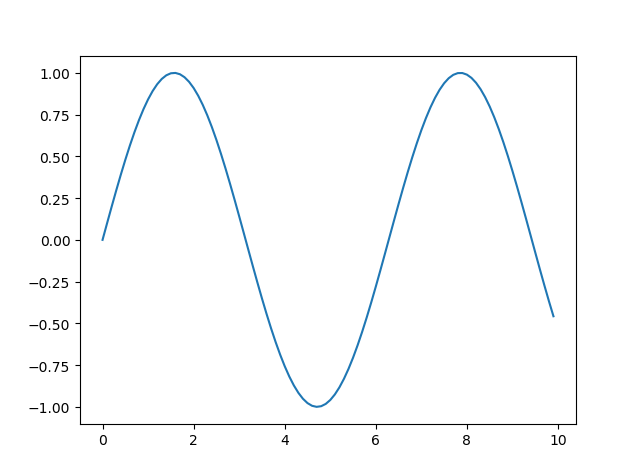
\includegraphics[scale=0.7]{figure/sinx.png}
  \caption{$y=sin(x)$ 的 Python 图像}\label{fig:sinx}
\end{figure}

\begin{center}
\begin{tcolorbox}[title = plot 函数的语法]
\textbf{plot([x], y, [fmt], **kwargs)}
\tcblower
\vspace{10pt}

\begin{tcboutputlisting}
\begin{tabular}{>{\bfseries}ll}
  [x] &可选参数,横坐标轴数据\\
  y & 纵坐标轴数据\\

[fmt] &可选参数,字符串,定义图形的基本样式:颜色,点形,线形\\
**kwargs &不定长的关键字参数,用字典形式设置图形的其他属性
\end{tabular}
\end{tcboutputlisting}
\tcbuselistingtext

\end{tcolorbox}
\end{center}

[fmt] 的常用代码(包括颜色代码、点形代码、线形代码),由表 \ref{table:plotParams} 所示。

\begin{table}[ht]
  \centering
  \caption{Plot 函数中的颜色、点形、线性代码}\label{table:plotParams}
  \vspace{5pt}
  \begin{subtable}{.3\linewidth}
    \caption{Plot 函数的颜色代码}
  \begin{tabular}{ll}
    \toprule
    颜色代码 & 颜色\\
    \midrule
    \textquotesingle b\textquotesingle & 蓝色\\
    \textquotesingle r\textquotesingle & 红色\\
    \textquotesingle g\textquotesingle & 绿色 \\
    \textquotesingle k\textquotesingle & 黑色\\
    \textquotesingle w\textquotesingle & 白色\\
    \textquotesingle y\textquotesingle & 黄色 \\
    \bottomrule
  \end{tabular}
\end{subtable}
\begin{subtable}{.3\linewidth}
  \caption{Plot 函数的点形代码}
\begin{tabular}{ll}
  \toprule
  线形代码 & 线形\\
  \midrule
  \textquotesingle o\textquotesingle & 实心圆形\\
  \textquotesingle .\textquotesingle & 点形\\
  \textquotesingle +\textquotesingle & 十字形\\
  \textquotesingle *\textquotesingle & 星号 \\
    \textquotesingle +\textquotesingle & 加号 \\
  \textquotesingle x\textquotesingle & 叉号\\
  \bottomrule
\end{tabular}
\end{subtable}
  \begin{subtable}{.3\linewidth}
    \caption{Plot 函数的线形代码}
  \begin{tabular}{ll}
    \toprule
    线形代码 & 线形\\
    \midrule
    \textquotesingle -\textquotesingle & 实线\\
    \textquotesingle -{}-\textquotesingle & 虚线\\
    \textquotesingle -.\textquotesingle & 折线 \\
    \textquotesingle :\textquotesingle & 点线\\

    &\\
    \bottomrule
  \end{tabular}
\end{subtable}
\end{table}

**kwargs 的常用设置包括线条的粗细 linewidth,图像标签  label 等。下面一些 plot 函数的代码展示了 [x],[fmt],**Kwargs 的一些可选用法。

\clearpage

\begin{lstlisting}[Language= Python]
>>> plot(x, y)        # 根据横坐标数据 x 与纵坐标数据 y 画图,采用默认的颜色、点形与线性
>>> plot(y)           # 据纵坐标数据 y 画图,横坐标数据默认为从 0 到 N-1,步长为 1 的等差数组
>>> plot(x, y, 'bo')  # 颜色为蓝色('b')、点形为圆('o')
>>> plot(y, 'g-.')     # 颜色为绿色('g'),线形为折线('-.')
>>> plt.plot(x, y, 'yo:', label='y=sin(x)', linewidth=2) # 颜色为黄色('y'),点形为圆形('o'),线形为虚线(':'),lable 内容为 'y=sin(x)', 线条宽度为 2
\end{lstlisting}


如果我们想自定义坐标轴的标题,坐标轴的刻度,坐标轴刻度的范围,设置图形标题,添加图例时,可以通过设置 pyplot 函数中的 xlable(横坐标轴标题), ylabel(纵坐标轴标题), xticks(横坐标轴刻度),yticks(纵坐标轴刻度),title(图形标题), grid(显示网格),legend(显示图例)等属性来实现。经过自定义设置,对图 \ref{fig:sinx} 的代码进行一下修改,生成图 \ref{fig:sinx2}。


\begin{lstlisting}[Language = Python]
# 导入宏包
import matplotlib.pyplot as plt
import numpy as np

# 这两行代码使得 pyplot 画出的图形中可以显示中文
plt.rcParams['font.sans-serif'] = ['SimHei']
plt.rcParams['axes.unicode_minus'] = False

# 生成数据
x = np.arange(0, 10, 0.5)
y = np.sin(x)

# 生成图形
plt.plot(x, y, 'go:', label='y=sin(x)', linewidth=2) # 颜色绿色,点形圆形,线性虚线,设置图例显示内容,线条宽度为2

plt.ylabel('y') # 横坐标轴的标题
plt.xlabel('x') # 纵坐标轴的标题
plt.xticks(np.arange(0, 11, 1)) # 设置横坐标轴的刻度为 0 到 10 的数组
plt.ylim([-2, 2]) # 设置纵坐标轴范围为 -2 到 2
plt.legend() # 显示图例, 图例中内容由 label 定义
plt.grid() # 显示网格
plt.title('我的第一个 Python 图形') # 图形的标题

# 显示图形
plt.show()

\end{lstlisting}

\begin{figure}[!ht]
  \centering
  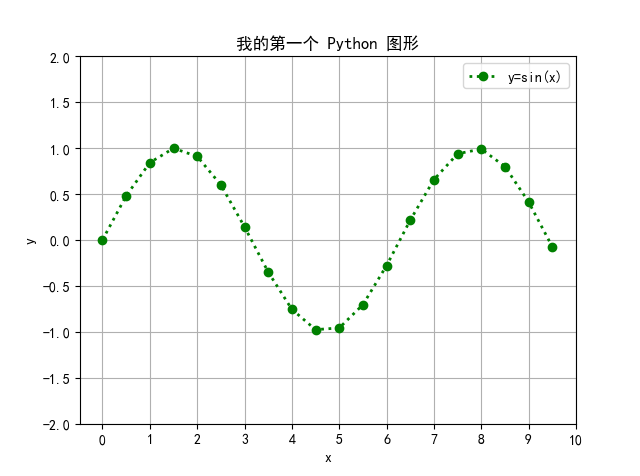
\includegraphics[width=\textwidth]{figure/sinx2.png}
  \caption{自定义坐标轴标题、刻度、范围,显示图例、网格与图形标题}\label{fig:sinx2}
\end{figure}


\section{线图}

在统计学中,线图一般用来表示时间序列数据,线图称为趋势图(run chart),因为从线图中可以清晰地看出数据虽时间变化的趋势。 表 \ref{table:GDP} 是我国近10年的 GDP 增长率,以及三大产业在近10年的增长率。


\begin{table}[!ht]
\centering
\renewcommand{\arraystretch}{1.2}
\caption{我国近10年的经济增长率, 数据来源:国家统计局}\label{table:GDP}
\begin{tabular}{|l|l|l|l|l|}
\hline

时间 & GDP增长率 & 第一产业增长率 & 第二产业增长率 & 第三产业增长率 \\ \hline
2009年 & 9.40  & 4.00  & 10.30  & 9.60  \\ \hline
2010年 & 10.60  & 4.30  & 12.70  & 9.70  \\ \hline
2011年 & 9.60  & 4.20  & 10.70  & 9.50  \\ \hline
2012年 & 7.90  & 4.50  & 8.40  & 8.00  \\ \hline
2013年 & 7.80  & 3.80  & 8.00  & 8.30  \\ \hline
2014年 & 7.30  & 4.10  & 7.40  & 7.80  \\ \hline
2015年 & 6.90  & 3.90  & 6.20  & 8.20  \\ \hline
2016年 & 6.70  & 3.30  & 6.30  & 7.70  \\ \hline
2017年 & 6.80  & 4.00  & 5.90  & 7.90  \\ \hline
2018年 & 6.60  & 3.50  & 5.80  & 7.60 \\ \hline
\end{tabular}
\end{table}



在画图时,横坐标轴数据为年份,纵坐标轴数据分别为 GDP 增长率,第一产业增长率,第二产业增长率,第三产业增长率。为了将四个纵坐标轴数据显示在一个图形上,可以用四个 plot 函数进行划线。Python 画图的代码为:

\begin{lstlisting}[Language = Python]
import matplotlib.pyplot as plt

# 这两行代码解决 plt 中文显示的问题
plt.rcParams['font.sans-serif'] = ['SimHei']
plt.rcParams['axes.unicode_minus'] = False

# 输入纵坐标轴数据与横坐标轴数据
gdp_rate = [9.4, 10.6, 9.6, 7.9, 7.8, 7.3, 6.9, 6.7, 6.8, 6.6]
first_industry_rate = [4.0, 4.3, 4.2, 4.50, 3.8, 4.1, 3.9, 3.3, 4.0, 3.5]
second_industry_rate = [10.3, 12.7, 10.7, 8.4, 8.0, 7.4, 6.2, 6.3, 5.9, 5.8]
third_industry_rate = [9.6, 9.7, 9.5, 8.0, 8.3, 7.8, 8.2, 7.7, 7.9, 7.6]
years = [2009, 2010, 2011, 2012, 2013, 2014, 2015, 2016, 2017, 2018]

# 4 个 plot 函数画出 4 条线,线形为折线,每条线对应各自的标签 label
plt.plot(years, gdp_rate, '.-', label='GDP增长率')
plt.plot(years, first_industry_rate, '.-', label='第一产业增长率')
plt.plot(years, second_industry_rate, '.-', label='第二产业增长率')
plt.plot(years, third_industry_rate, '.-', label='第三产业增长率')

plt.xticks(years)  # 设置横坐标刻度为给定的年份
plt.xlabel('年份') # 设置横坐标轴标题
plt.legend() # 显示图例,即每条线对应 label 中的内容
plt.show() # 显示图形
\end{lstlisting}

显示效果如图 \ref{fig:gdp} 所示。

\begin{figure}[!ht]
\centering
  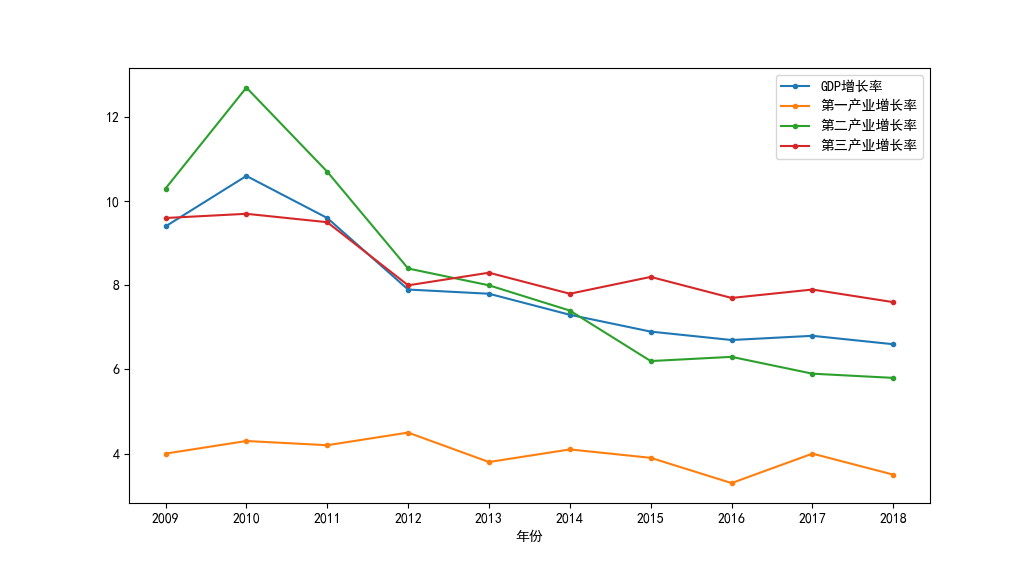
\includegraphics[width=\textwidth]{figure/gdp.png}
  \caption{近十年我国的 GDP 以及各产业增长率}\label{fig:gdp}
\end{figure}

\section{散点图}

散点图是数据点在直角坐标系平面上的分布图,在统计学的回归分析与预测中经常用到。用横轴代表变量 $x$,纵轴代表变量 $y$,每组数据 $(x_i, y_i)$ 在坐标系中用一个点表示。
做散点图要用到 pyplot 中的 scatter 函数,该函数的基本语法为\footnote{在 matplotlib 宏包中,0 到 1 之间的浮点数产生相应的 RGB 颜色}:

\begin{center}
\begin{tcolorbox}[title = scatter 函数的语法]
\textbf{scatter(x, y, [s], [c], **kwargs)}
\tcblower
\vspace{10pt}

\begin{tcboutputlisting}
\begin{tabular}{>{\bfseries}ll}
  x &横坐标轴数据\\
  y & 纵坐标轴数据\\

[s] &可选参数,一个数或一个数组,设置每个散点的大小\\

[c] &可选参数,一个数或一个数组,设置每个散点的颜色\\
**kwargs &不定长的关键字参数,用字典形式设置图形的其他属性
\end{tabular}
\end{tcboutputlisting}
\tcbuselistingtext

\end{tcolorbox}
\end{center}

**kwargs 中常设置的是不透明度属性 alpha,其大小为0到1之间的浮点数。假设某个农产品的产量与温度和降雨量的关系如表 \ref{table:scatter} 所示。

\begin{table}[!ht]
\centering
\renewcommand{\arraystretch}{1.2}
\caption{某农产品的产量与温度和降雨量的关系}\label{table:scatter}
\begin{tabular}{|l|l|l|l|}
\hline
产量 & 温度 & 降雨量 \\ \hline
1125 & 6 & 25 \\ \hline
1725 & 8 & 40 \\ \hline
2250 & 10 & 58 \\ \hline
2875 & 13 & 68 \\ \hline
2900 & 14 & 110 \\ \hline
3750 & 16 & 98 \\ \hline
4125 & 21 & 120 \\ \hline

\end{tabular}
\end{table}

作出产量与温度的散点图的 Python 代码与图形如下:
\begin{lstlisting}[Language=Python]
import matplotlib.pyplot as plt
import numpy as np

# 这两行代码解决 plt 中文显示的问题
plt.rcParams['font.sans-serif'] = ['SimHei']
plt.rcParams['axes.unicode_minus'] = False

# 输入产量与温度数据
production = [1125, 1725, 2250, 2875, 2900, 3750, 4125]
tem = [6, 8, 10, 13, 14, 16, 21]

colors = np.random.rand(len(tem))  # 颜色数组
plt.scatter(tem, production, s=200, c=colors)  # 画散点图,大小为 200
plt.xlabel('温度')  # 横坐标轴标题
plt.ylabel('产量')  # 纵坐标轴标题
plt.show()
\end{lstlisting}

\begin{figure}[!ht]
  \centering
  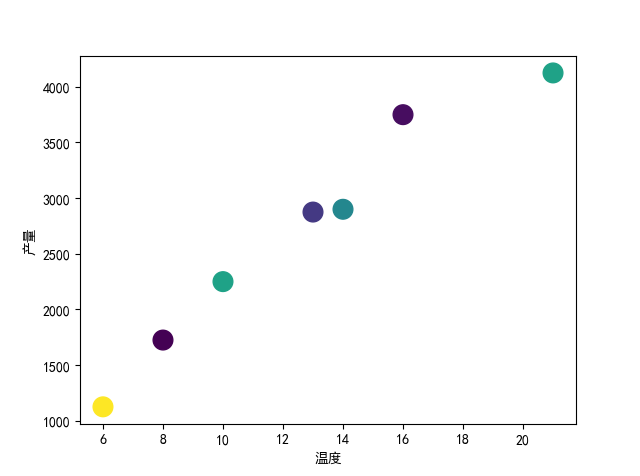
\includegraphics{figure/scatter1.png}
  \caption{产量与温度的散点图}
\end{figure}

若将散点大小的数据换为第三个变量的数值,则可以作出反映三个变量关系的气泡图。下面的代码和图形做出了一个气泡图。图 \ref{fig:scatter2} 反映了产量与温度、降雨量的关系:温度数值在横坐标轴,降雨量数值在纵坐标轴,降雨量的大小用气泡的大小表示。

\begin{lstlisting}[Language=Python]
import matplotlib.pyplot as plt
import numpy as np

# 这两行代码解决 plt 中文显示的问题
plt.rcParams['font.sans-serif'] = ['SimHei']
plt.rcParams['axes.unicode_minus'] = False

# 输入产量与温度数据
production = [1125, 1725, 2250, 2875, 2900, 3750, 4125]
tem = [6, 8, 10, 13, 14, 16, 21]
rain = [25, 40, 58, 68, 110, 98, 120]

colors = np.random.rand(len(tem))  # 颜色数组
size = production
plt.scatter(tem, rain, s=size, c=colors, alpha=0.6)  # 画散点图, alpha=0.6 表示不透明度为 0.6
plt.ylim([0, 150])  # 纵坐标轴范围
plt.xlim([0, 30])   # 横坐标轴范围
plt.xlabel('温度')  # 横坐标轴标题
plt.ylabel('降雨量')  # 纵坐标轴标题
plt.show()
\end{lstlisting}

\begin{figure}[!ht]
  \centering
  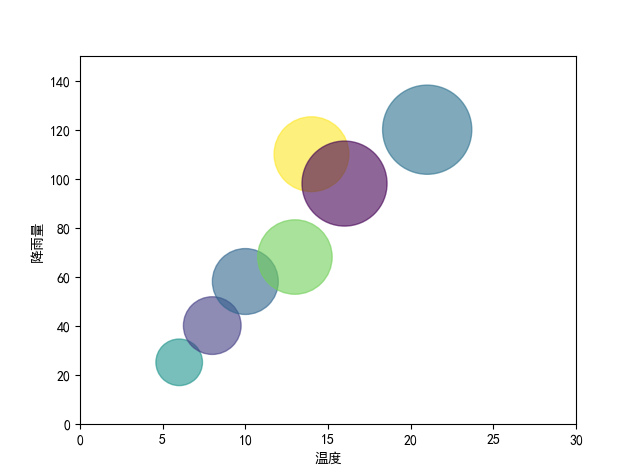
\includegraphics{figure/scatter2.png}
  \caption{产量与温度、降雨量关系的气泡图}\label{fig:scatter2}
\end{figure}

\clearpage

\section{条形图}

条形图(bar chart),也称为柱状图,是一种以长方形的长度为变量的统计图表,长方形的长度与它所对应的变量数值呈一定比例。画条形图要用到 pyplot 中的 bar 函数,该函数的基本语法为:

\begin{center}
\begin{tcolorbox}[title = bar 函数的语法]
\textbf{bar(x, height, [width],  **kwargs)}
\tcblower
\vspace{10pt}

\begin{tcboutputlisting}
\begin{tabular}{>{\bfseries}ll}
  x &数组,每个条形的横坐标\\
  height & 一个数或一个数组,条形的高度\\

[width] &可选参数,一个数或一个数组,条形的宽度,默认为 0.8\\

**kwargs &不定长的关键字参数,用字典形式设置条形图的其他属性
\end{tabular}
\end{tcboutputlisting}
\tcbuselistingtext
\end{tcolorbox}
\end{center}

**kwargs 中常设置的参数包括图形标签 label,颜色标签 color,不透明度 alpha 等。假设某项针对男女大学生购买饮用水爱好的调查结果如下表:

\begin{table}[!ht]
\centering
\caption{男女大学生购买饮用水爱好调查表}
\renewcommand{\arraystretch}{1.2}
\begin{tabular}{|l|l|l|l|}
\hline
买水选择 & 男 & 女 \\ \hline
碳酸饮料 & 6 & 9 \\ \hline
绿茶 & 7 & 4 \\ \hline
矿泉水 & 6 & 4 \\ \hline
果汁 & 1 & 5 \\ \hline
其他 & 2 & 6 \\ \hline
总计 & 22 & 28 \\ \hline
\end{tabular}
\end{table}

画出男生饮用水情况的直方图,代码如下:

\begin{lstlisting}[Language=Python]
import matplotlib.pyplot as plt

# 这两行代码解决 plt 中文显示的问题
plt.rcParams['font.sans-serif'] = ['SimHei']
plt.rcParams['axes.unicode_minus'] = False

waters = ('碳酸饮料', '绿茶', '矿泉水', '果汁', '其他')
buy_number = [6, 7, 6, 1, 2]

plt.bar(waters, buy_number)
plt.title('男性购买饮用水情况的调查结果')

plt.show()
\end{lstlisting}

显示的图形:
\begin{figure}[!ht]
  \centering
  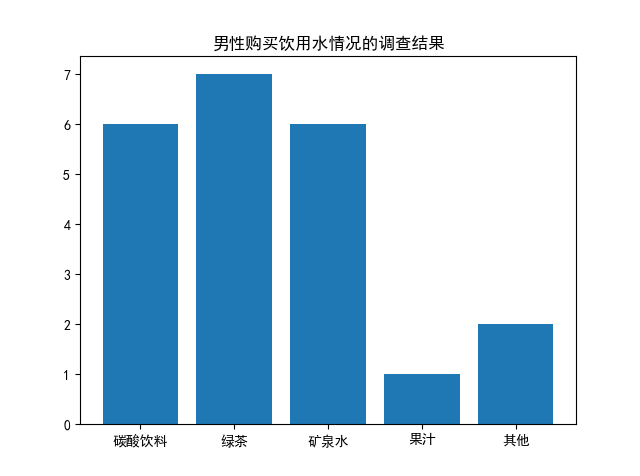
\includegraphics[scale=0.8]{figure/bar1.png}
  \caption{男性购买饮用水条形图}
\end{figure}


若要生成横的条形图,则可以使用 barh 函数,其语法与 bar 函数非常类似。

\begin{center}
\begin{tcolorbox}[title = barh 函数的语法]
\textbf{bar(x, width, [height], **kwargs)}
\tcblower
\vspace{10pt}

\begin{tcboutputlisting}
\begin{tabular}{>{\bfseries}ll}
    y &数组,每个条形的纵坐标\\
    width & 一个数或一个数组,条形的宽度\\

  [height] &可选参数,一个数或一个数组,条形的高度,默认为 0.8\\

**kwargs &不定长的关键字参数,用字典形式设置条形图的其他属性
\end{tabular}
\end{tcboutputlisting}
\tcbuselistingtext
\end{tcolorbox}
\end{center}

对应的代码与图形为:

\begin{lstlisting}[Language=Python]
import matplotlib.pyplot as plt

# 这两行代码解决 plt 中文显示的问题
plt.rcParams['font.sans-serif'] = ['SimHei']
plt.rcParams['axes.unicode_minus'] = False

waters = ('碳酸饮料', '绿茶', '矿泉水', '果汁', '其他')
buy_number = [6, 7, 6, 1, 2]

plt.barh(waters, buy_number)  # 横放条形图函数 barh
plt.title('男性购买饮用水情况的调查结果')

plt.show()
\end{lstlisting}

\begin{figure}[!ht]
  \centering
  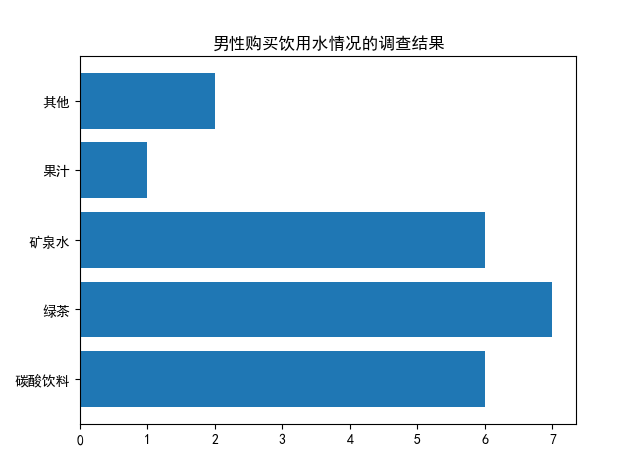
\includegraphics[scale=0.8]{figure/bar2.png}
  \caption{男性购买饮用水条形图(条形横放)}\label{fig:bar2}
\end{figure}



若要将男生与女生的调查情况画出两个条形图一块显示,则可以使用 bar 或 barh 函数两次,并调整 bar 或 barh 函数的条形图位置坐标以及相应刻度,使得两组条形图能够并排显示。

\begin{lstlisting}[Language=Python]
import matplotlib.pyplot as plt
import numpy as np

# 这两行代码解决 plt 中文显示的问题
plt.rcParams['font.sans-serif'] = ['SimHei']
plt.rcParams['axes.unicode_minus'] = False

# 输入统计数据
waters = ('碳酸饮料', '绿茶', '矿泉水', '果汁', '其他')
buy_number_male = [6, 7, 6, 1, 2]
buy_number_female = [9, 4, 4, 5, 6]

bar_width = 0.3  # 条形宽度
index_male = np.arange(len(waters))  # 男生条形图的横坐标
index_female = index_male + bar_width  # 女生条形图的横坐标

# 使用两次 bar 函数画出两组条形图
plt.bar(index_male, height=buy_number_male, width=bar_width, color='b', label='男性')
plt.bar(index_female, height=buy_number_female, width=bar_width, color='g', label='女性')

plt.legend()  # 显示图例
plt.xticks(index_male + bar_width/2, waters)  # 让横坐标轴刻度显示 waters 里的饮用水, index_male + bar_width/2 为横坐标轴刻度的位置
plt.ylabel('购买量')  # 纵坐标轴标题
plt.title('购买饮用水情况的调查结果')  # 图形标题

plt.show()
\end{lstlisting}

生成图 \ref{fig:bar3}。
\begin{figure}[!ht]
  \centering
  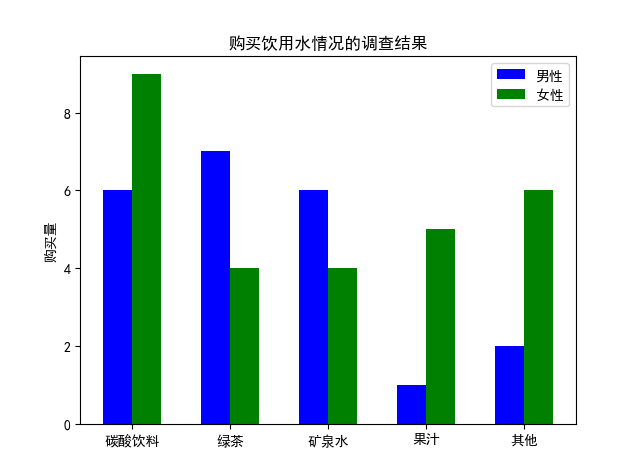
\includegraphics[scale=0.8]{figure/bar3.png}
  \caption{男女购买饮用水条形图}\label{fig:bar3}
\end{figure}

\clearpage
\section{直方图}

直方图(histogram)虽然在样式上类似条形图,但它们的作用不一样。直方图用不同的矩形表示频数,常用来观察一组数据的概率分布。在直角坐标中,用横轴表示数据分组,纵轴表示频数或频率,各组与相应的频数就形成了一个个矩形,即直方图。

画直方图用到 pyplot 中的 hist 函数,它的基本语法为:

\begin{center}
\begin{tcolorbox}[title = hist 函数的语法]
\textbf{[n, bins, patches] = hist(x, [bins], **kwargs)}
\tcblower
\vspace{5pt}

\begin{tcboutputlisting}
\begin{tabular}{>{\bfseries}ll}
  \textbf{输入值:}&\\
    x &数组,需要绘制直方图的数值\\

  [bins] &可选参数,数据的组数,若不指定则 hist 函数默认计算一个组数\\

**kwargs &不定长的关键字参数,用字典形式设置条形图的其他属性\\
&\\
  \textbf{返回值:} &\\
n &一个数组,每组直方图的频数(或概率密度)\\
bins &一个数组,直方图的边界数值\\
patches & 一个对象组,每个对象代表直方图的矩形

\end{tabular}

\tcblower

\end{tcboutputlisting}
\tcbuselistingtext
\end{tcolorbox}
\end{center}

**kwargs 中常用来设置的属性包括直方的边界线颜色 edgecolor,不透明度 alpha 等。需要注意的是,hist 函数的三个返回值一般用来继续对数据进行分析,并不是必须要写或必须要使用的。下面举例说明该函数,例如某个饭店每天接待的顾客数有以下记录值:

\begin{table}[!ht]
\centering
\renewcommand{\arraystretch}{1.2}
\caption{某饭店每天接待的顾客数的记录值}
\begin{tabular}{|l|l|l|l|l|l|l|l|l|l|}
\hline

141 & 159 & 166 & 172 & 177 & 182 & 188 & 196 & 203 & 214 \\ \hline
143 & 160 & 167 & 173 & 177 & 183 & 189 & 196 & 203 & 215 \\ \hline
144 & 160 & 168 & 173 & 178 & 184 & 189 & 196 & 205 & 218 \\ \hline
149 & 161 & 168 & 174 & 178 & 185 & 189 & 196 & 206 & 223 \\ \hline
150 & 161 & 168 & 174 & 178 & 186 & 190 & 196 & 207 & 225 \\ \hline
152 & 162 & 170 & 174 & 179 & 186 & 190 & 197 & 208 & 226 \\ \hline
153 & 163 & 171 & 175 & 179 & 187 & 191 & 197 & 209 & 228 \\ \hline
153 & 163 & 171 & 175 & 179 & 187 & 192 & 198 & 210 & 233 \\ \hline
154 & 164 & 172 & 175 & 180 & 187 & 194 & 198 & 210 & 233 \\ \hline
155 & 165 & 172 & 175 & 180 & 187 & 194 & 200 & 211 & 234 \\ \hline
156 & 165 & 172 & 176 & 181 & 188 & 195 & 201 & 211 & 234 \\ \hline
158 & 165 & 172 & 176 & 182 & 188 & 195 & 202 & 213 & 237 \\ \hline

\end{tabular}
\end{table}

在 Phthon 中编写代码,并画出对应的直方图。

\clearpage
\begin{lstlisting}[Language=Python]
import matplotlib.pyplot as plt

x = [141, 159, 166, 172, 177, 182, 188, 196, 203, 214,
     143, 160, 167, 173, 177, 183, 189, 196, 203, 215,
     144, 160, 168, 173, 178, 184, 189, 196, 205, 218,
     149, 161, 168, 174, 178, 185, 189, 196, 206, 223,
     150, 161, 168, 174, 178, 186, 190, 196, 207, 225,
     152, 162, 170, 174, 179, 186, 190, 197, 208, 226,
     153, 163, 171, 175, 179, 187, 191, 197, 209, 228,
     153, 163, 171, 175, 179, 187, 192, 198, 210, 233,
     154, 164, 172, 175, 180, 187, 194, 198, 210, 233,
     155, 165, 172, 175, 180, 187, 194, 200, 211, 234,
     156, 165, 172, 176, 181, 188, 195, 201, 211, 234,
     158, 165, 172, 176, 182, 188, 195, 202, 213, 237]

plt.hist(x, edgecolor='k', alpha=0.35) # 设置直方边线颜色为黑色,不透明度为 0.35
plt.show()
\end{lstlisting}

\begin{figure}[!ht]
  \centering
  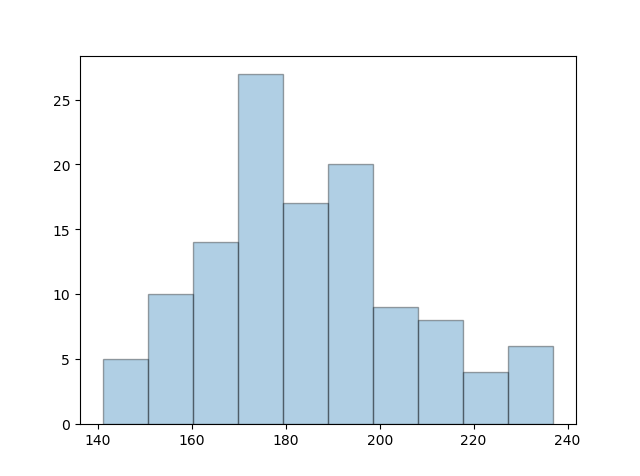
\includegraphics[scale=0.8]{figure/hist.png}
  \caption{每天接待顾客数分布的直方图}\label{fig:hist}
\end{figure}

从图 \ref{fig:hist} 可以看出,每天的顾客数大致符合一个正态分布。

\section{饼图}

饼图(pie char)是一个划分为几个扇形的圆形统计图表,一般用于描述频率或百分比之间的相对关系。在饼图中,每个扇区的弧长(以及圆心角和面积)的大小与其所表示的数量呈固定比例。

画饼图一般使用 pyplot 中的 pie 函数,它的基本语法如下:

\begin{center}
\begin{tcolorbox}[title = pie 函数的语法]
\textbf{bar(x, [expode], [labels], [autopic], **kwargs)}
\tcblower
\vspace{10pt}

\begin{tcboutputlisting}
\begin{tabular}{>{\bfseries}ll}
    x &数组,每个扇区的比例\\

    [expode] & 可选参数,数组,每个扇区突出的大小\\

  [labels] &可选参数,字符串数组,每个扇区的标签\\

  [autopct] &可选参数,字符串或函数,每个扇区显示的数字样式\\

**kwargs &不定长的关键字参数,用字典形式设置条形图的其他属性
\end{tabular}
\end{tcboutputlisting}
\tcbuselistingtext
\end{tcolorbox}
\end{center}

**kwargs 中常用来设置的属性包括是否显示扇区的阴影 shadow, 扇区的起始角度 startangle 等。假设有下列调查数据:

\begin{table}[!ht]
\centering
\renewcommand{\arraystretch}{1.2}
\caption{购水类型的调查数据}
\begin{tabular}{|l|l|}
\hline

购水类型 & 人数 \\ \hline
碳酸饮料 & 15 \\ \hline
绿茶 & 11 \\ \hline
矿泉水 & 10 \\ \hline
其他 & 8 \\ \hline
果汁 & 6 \\ \hline

\end{tabular}
\end{table}

饼图的代码与图形:

\begin{lstlisting}[Language=Python]
import matplotlib.pyplot as plt
import numpy as np

# 这两行代码解决 plt 中文显示的问题
plt.rcParams['font.sans-serif'] = ['SimHei']
plt.rcParams['axes.unicode_minus'] = False

labels = ['果汁', '矿泉水', '绿茶', '其他', '碳酸饮料']
x = [6, 10, 11, 8, 15]
explode = [0, 0.1, 0, 0, 0]  # 突出显示第二个扇区

plt.pie(x, explode=explode, labels=labels, autopct='%.2f%%', shadow=True, startangle=90)
plt.legend()  # 显示标签
plt.axis('equal')  # 让图形和坐标轴相等,这样避免饼图为椭圆形
plt.show()
\end{lstlisting}

\begin{figure}[!ht]
  \centering
  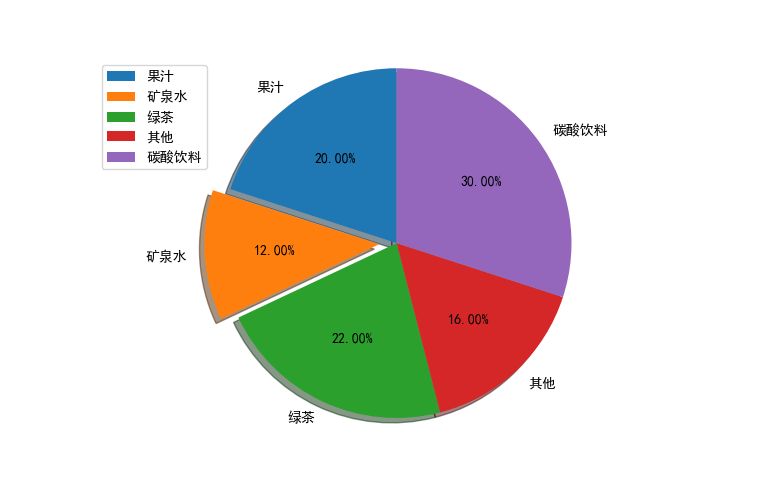
\includegraphics[scale=0.7]{figure/pie1.png}
  \caption{调查结果的饼图}\label{fig:pie}
\end{figure}

若在饼图上既要显示比率,又要显示实际调查数字,则可以通过自定义 autopct 函数来实现:
\begin{lstlisting}[Language=Python]
import matplotlib.pyplot as plt
import numpy as np

# 这两行代码解决 plt 中文显示的问题
plt.rcParams['font.sans-serif'] = ['SimHei']
plt.rcParams['axes.unicode_minus'] = False


# 自定义 autopct 函数
def func(pct, allvals):
    absolute = int(round(pct*np.sum(allvals)/100.0))
    return "{:.1f}%\n({:d})".format(pct, absolute)


labels = ['果汁', '矿泉水', '绿茶', '其他', '碳酸饮料']
x = [6, 10, 11, 8, 15]
explode = [0, 0.1, 0, 0, 0]  # 突出显示第二个扇区

plt.pie(x, explode=explode, labels=labels, autopct=lambda pct: func(pct, x),  # 利用 lambda 定义 pct 函数
        shadow=True, startangle=90)
plt.legend()  # 显示标签
plt.axis('equal')  # 让图形和坐标轴相等,这样饼图会更好看
plt.show()
\end{lstlisting}

\begin{figure}[!ht]
  \centering
  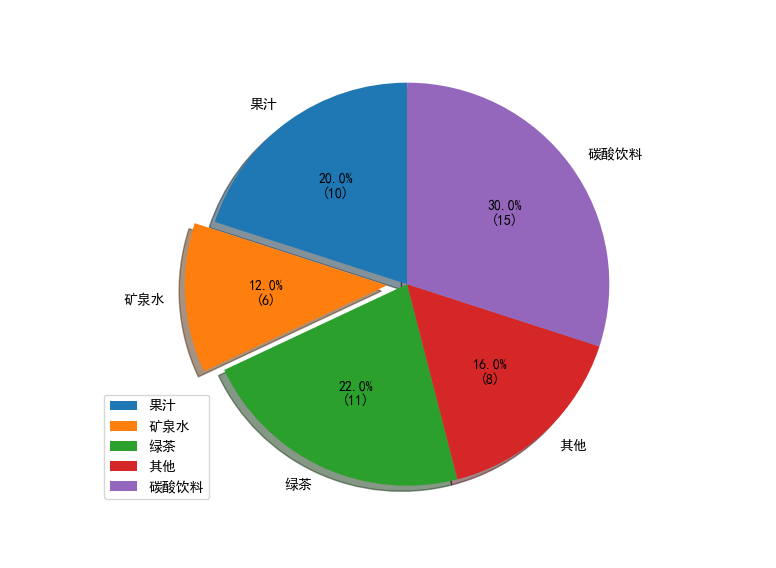
\includegraphics[scale=0.7]{figure/pie2.png}
  \caption{调查结果的饼图(同事显示比例与原始数据)}\label{fig:pie}
\end{figure}

\clearpage
\section{箱线图}

箱线图(box plot)在学术论文中经常出现,是一种用来显示一组数据分散情况资料的统计图,由数据的最大值、最小值、中位数、两个四分位数,共五个特征绘制而成。


\begin{table}[!ht]
\centering
\caption{学生成绩统计表}
\begin{tabular}{|l|l|l|l|l|l|l|l|l|l|l|l|}
\hline
&\multicolumn{11}{c|}{学生编号}  \\\hline
课程名称 & 1 & 2 & 3 & 4 & 5 & 6 & 7 & 8 & 9 & 10 & 11 \\ \hline
英语 & 76 & 90 & 97 & 71 & 70 & 93 & 86 & 83 & 78 & 85 & 81 \\ \hline
西方经济学 & 93 & 81 & 76 & 88 & 66 & 79 & 83 & 92 & 78 & 86 & 78 \\ \hline
市场营销学 & 74 & 87 & 85 & 69 & 90 & 80 & 77 & 84 & 91 & 74 & 70 \\ \hline
财务管理 & 68 & 75 & 70 & 84 & 73 & 60 & 76 & 81 & 88 & 68 & 75 \\ \hline
统计学 & 55 & 91 & 68 & 73 & 84 & 81 & 70 & 69 & 94 & 62 & 71 \\ \hline

\end{tabular}
\end{table}
